\documentclass[a4paper,12pt,spanish]{article}
\usepackage[spanish,activeacute]{babel}
\usepackage[utf8]{inputenc}
\usepackage{tocbibind}
\usepackage[colorlinks=true,linkcolor=blue]{hyperref}
\usepackage{eurosym}
\usepackage{listings}
\usepackage{color}
\usepackage{fancyvrb}
\usepackage{times}
\usepackage{sans}

\definecolor{gray97}{gray}{.95}
\definecolor{gray75}{gray}{.75}
\definecolor{gray45}{gray}{.45}

\lstset{ frame=Ltb,
     framerule=0pt,
     aboveskip=0.5cm,
     framextopmargin=3pt,
     framexbottommargin=3pt,
     framexleftmargin=0.4cm,
     framesep=0pt,
     rulesep=.4pt,
     backgroundcolor=\color{gray97},
     rulesepcolor=\color{black},
     %
     stringstyle=\ttfamily,
     showstringspaces = false,
     basicstyle=\small\ttfamily,
     commentstyle=\color{gray45},
     keywordstyle=\bfseries,
     %
     numbers=left,
     numbersep=15pt,
     numberstyle=\tiny,
     numberfirstline = false,
     breaklines=true,
   }

% minimizar fragmentado de listados
\lstnewenvironment{listing}[1][]
   {\lstset{#1}\pagebreak[0]}{\pagebreak[0]}

\lstdefinestyle{consola}
   {basicstyle=\scriptsize\bf\ttfamily,
    backgroundcolor=\color{gray75},
   }
 
\lstdefinestyle{Java}
   {language=Java,
   }

\RequirePackage{ifpdf} % ¿latex o pdflatex?
% Configuración de las imágenes
\ifpdf
	\usepackage[pdftex]{graphicx}	% Inclusión de imágenes
	\DeclareGraphicsExtensions{.pdf,.png,.jpg}
\else
	\usepackage{graphicx}		% Inclusión de imágenes
	\DeclareGraphicsExtensions{.eps}
\fi
\graphicspath{ {./img/} } % Ruta respecto al fichero tex principal dónde se buscan

\oddsidemargin 0in
\textwidth 6.5in
\topmargin -0.5in
\textheight 9.5in
\parindent 0em

\author{Adrián Cepillo Macías}
\title{Tutorial de Introducción a Grails}

\begin{document}
\begin{titlepage}
  \maketitle
  \begin{figure}[h!]
    \centering
    \vspace{1in}
    
\includegraphics[scale=0.65]{grailsportada}
    \label{fig:Portada}
  \end{figure}
\end{titlepage}
 
\tableofcontents
\newpage 

\section{Instalación de Grails}
Siguiendo con el tutorial anterior ahora vamos a instalar Grails de nuevo manualmente. Primero descargar la aplicacion desde \href{http://grails.org/Download}{aquí.} La extraemos en el directorio que prefiramos.\\

Luego establecer una variable de entorno:
\begin{itemize}
\item \$ export GRAILS\_HOME=~/RUTA\_EXTRACCION/bin
\end{itemize}

Podemos hacer esto permanente introduciendo este comando al final del fichero ~/.bashrc.\\

Aún así nosotros no usaremos grails por consola, se muestra esta instalación por si se quiere usar grails independientemente de eclipse. Nosotros veremos en este tutorial algunos de los comandos que grails contiene para crear una aplicacion, testearla, ... pero todo desde el prompt que nos ofrece Eclipse.

\section{Creando nuestra aplicación}
Vamos a crear de nuevo la aplicación {\it Book}. Creamos un nuevo proyecto, esta vez elegiremos una instalación específica. Para ello debemos clickar en {\it Configure Grails Installations} y añadiremos la versión que acabamos de descargarnos, indicando el directorio en el que se encuentra.\\

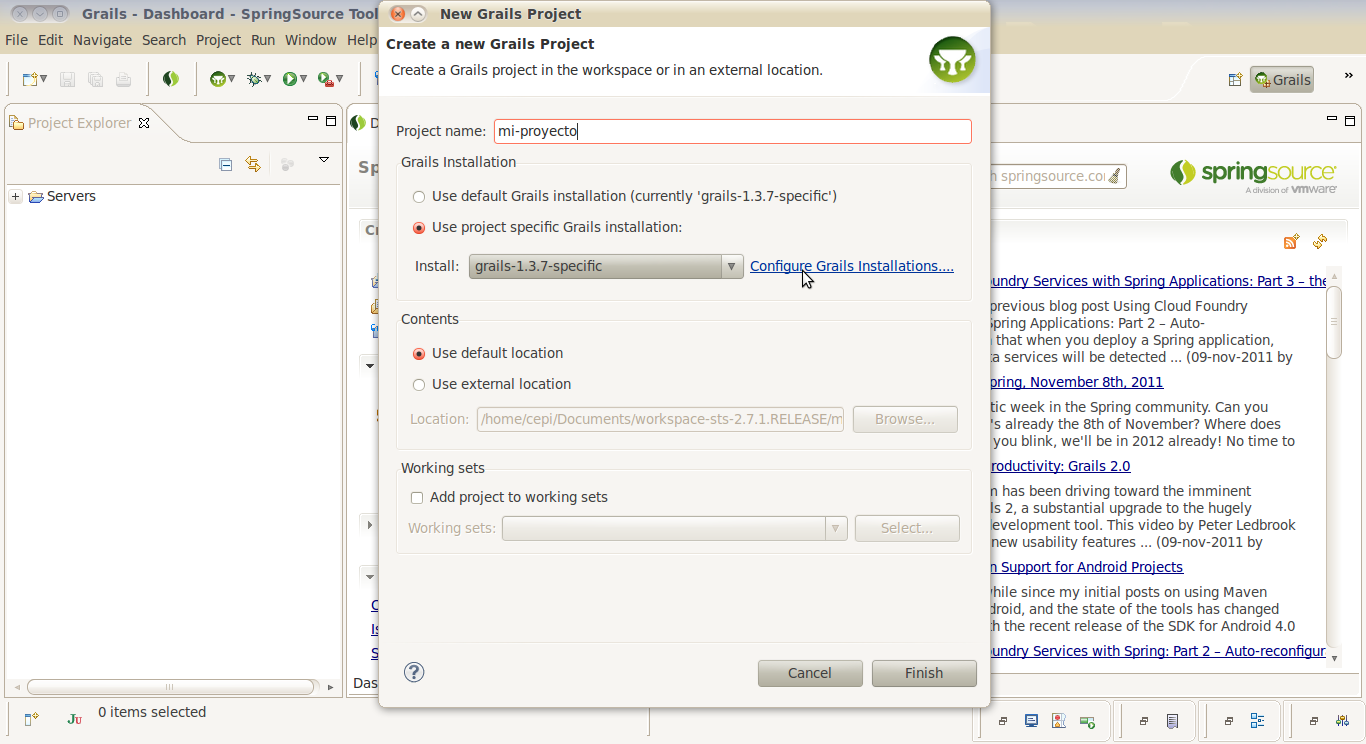
\includegraphics[scale=0.35]{proyecto-specific}\\

{\bf Nota:} El comando de {\it Grails} para crear un proyecto es, {\bf \$ grails create-app mi-proyecto}. {\it Eclipse} no permite crear un proyecto, introduciendo este comando en el prompt.\\

Para conocer algunos de los comandos de {\it Grails} vamos a usar el prompt que nos presenta {\it Eclipse STS}. Podemos encontrarlo en Navigate-$>$Open Grails Commands Prompt. O clickar en el simbolo de {\it Grails} en la barra de herramientas o pulsar Ctrl+Alt+Shift+G (Cmd+Alt+Shift+G en Mac). Con Ctrl+Space (Cmd+Space) nos mostrará el asistente.\\

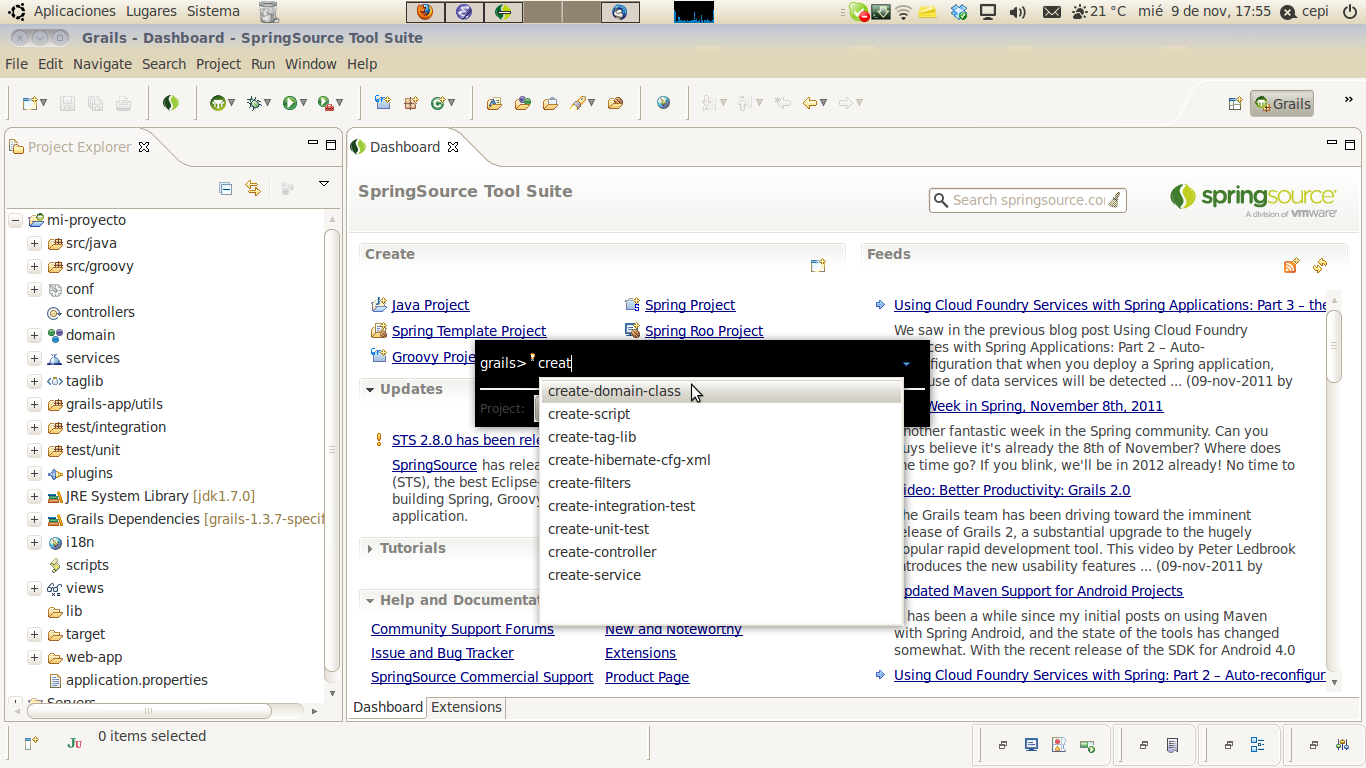
\includegraphics[scale=0.35]{create-domain}\\
 
Ahora crearemos la clase de dominio introduciendo en el prompt:
\begin{itemize}
\item grails$>$ create-domain-class org.example.Book
\end{itemize}

Modificamos el código:\\

\lstinputlisting[style=Java]{resources/Book.groovy}

Y lo mismo para el controlador:
\begin{itemize}
\item grails$>$ create-controller org.example.Book
\end{itemize}

\lstinputlisting[style=Java]{resources/BookController.groovy}

Corremos la aplicación ejecutando:
\begin{itemize}
\item grails$>$ run-app
\end{itemize}

\section{Importando datos de prueba}
Es probable que queramos probar la aplicación con ciertos datos y sería muy pesado tener que introducirlos a mano una y otra vez. Para ello podemos modificar el fichero de configuración {\it BootStrap.groovy}, dentro de {\it conf} en la jerarquía del proyecto.

\lstinputlisting[style=Java]{resources/BootStrap.groovy}

Como podemos comprobar hemos redefinido {\it init} de esta forma cada vez que se inicie la aplicación se importaran estos datos a el modelo señalado.\\ 

Debemos notar la llamada a {\it Book.count()}. Este método devuelve el número de libros que existen ya en la base de datos. Con el {\it if()\{...\}} decimos que en caso que no existan otros datos de testeo, se introduzcan estos datos.\\

Por otra parte, llamamos al método {\it Book.save()}, el cuál guarda el objeto en la base de datos. Y establecemos la opción {\it failOnError: true} indicando que se lance una excepción en caso que el método falle.

\section{Configuración del Data Source}

Hasta ahora hemos estado trabajando con la base de datos HSQLDB en memoria, para desarrollo y testeo. Vamos a configurar una base de datos alternativa. Para ello modificamos el fichero {\it DataSource.groovy.}

\lstinputlisting[style=Java]{resources/DataSource.groovy}

En este caso estamos usando Mysql. Grails ya tiene el driver para JDBC pero es necesario descomentar varias líneas del fichero {\it BuildConfig.groovy}.

\lstinputlisting[style=Java]{resources/BuildConfig.groovy}

\section{Ampliando nuestra aplicación}
\subsection{Creando la clase Author}

Vamos a añadir algunos elementos nuevos a la aplicación empezando por crear otra clase llamada {\it Author} que relacionar con {\it Book}. Se muestra primero el código de la {\it domain class}:

\lstinputlisting[style=Java]{resources/Author.groovy}

Y por otra parte el controlador:

\lstinputlisting[style=Java]{resources/AuthorController.groovy}

\subsection{Relacionando con GORM}

\lstinputlisting[style=Java]{resources/AuthorGORM.groovy}

\lstinputlisting[style=Java]{resources/BookGORM.groovy}

\subsection{Modificando un controlador generado}
\subsection{Cambiemos de estilo}
\end{document}
